\documentclass[a4paper,UTF8]{ctexart}

\usepackage{amsmath, amsthm, amssymb, amsfonts, hyperref, mathrsfs}%美国数学学会的包+?
\usepackage{geometry} %控制界面
\usepackage{bookmark}
\usepackage{fancyhdr} % header & footer
\usepackage{appendix} % 附录
\usepackage{tikz} %作图
\usepackage{graphicx} %插入图片的宏包
\usepackage{float} %设置图片浮动位置的宏包
\usepackage{subfigure} %插入多图时用子图显示的宏包
\usepackage{listings} %引用代码
\usepackage{physics,mathtools} %物理数学工具
\usepackage{comment}
\usepackage{framed}
\geometry{top=2.5cm,bottom=2.5cm,left=2.5cm,right=2.5cm} % 布局要求
\pagestyle{fancy} % fancy分格
\fancyhf{} % 清除所有页眉页脚
\renewcommand\headrulewidth{0.6pt}
\renewcommand\footrulewidth{0.6pt}
\lhead{何金铭 PB21020660$\mid$座位号:5}
\chead{核磁共振实验报告}
\rhead{\thepage}
\lfoot{2023.4.25}
\rfoot{USTC}
%\bibliographystyle{plain} % 引用样式
\everymath{\displaystyle} % display
%============================================================

\begin{document}

\begin{center}
    \textbf{\Large 核磁共振实验报告}
    \par \text{\large 何金铭 PB21020660}
\end{center}

\begin{abstract}
    核磁共振是一个重要的物理现象,也有很多实际应用。本实验利用扫频法来做实现核磁共振,并且
    会利用一个简单的实验装置来测量H的$\gamma_{H},g_{H}$因子和$^{19}F$的$\gamma_{F},g_{F}$因子。
    并且利用了测得的$\gamma_H$来测量磁体于其它位置产生的$B_0$。最后测量了5个不同调制电压下的$B_m$
    \par\textbf{关键词:}核磁共振,扫频法,磁感应强度测量
\end{abstract}

\section{引言}

核磁共振是一个重要的物理现象,先简单叙述一下它的实验原理。

\subsection{实验原理}

\begin{comment}

\begin{figure}[H]
    \centering
    \begin{minipage}[b]{0.9\textwidth}
        \centering
        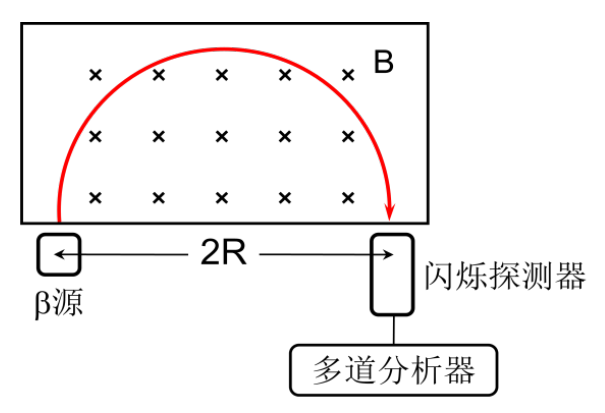
\includegraphics[width=0.4\textwidth]{./m.png}
        \caption{半圆聚焦$\beta$磁谱仪与闪烁能谱仪示意图}
    \end{minipage}
\end{figure}

\end{comment}

\subsubsection{Lamor进动}

由于原子核有轨道磁矩和自旋磁矩,故于外场$B_0$中会做进动,且有关系$\omega_0 = \gamma B_0$。
其中$\omega_0$称为Lamor频率,$\gamma = g \frac{q}{2m}$称为旋磁比,g为朗德因子

\subsubsection{磁共振}

于$x$-$y$平面中加入一个角频率与Lamor频率相同(即:$\omega=\omega_0=\gamma B_0$)的外加旋转磁场$B_1$中。此时,
磁矩与$B_1$相对静止,会使磁矩绕$B_1$产生进动,势能增加。

\begin{itemize}
    \item 对于电子自旋共振,$\gamma = g \frac{\mu_B}{\hbar }$
    \item 对于核自旋共振,$\gamma = g \frac{\mu_N}{\hbar}$
\end{itemize}

\subsubsection{塞曼分裂}

含自旋的原子核会在外磁场中产生能级分裂,在适当波长中的电磁波诱导下,不同能级之间会有跃迁,产生强弱不同的共振信号。

\subsubsection{检验共振信号}

一般有吸收法、感应法、平衡法等几种方法,不同的方法有不同的特点,这里不详细展开叙述。

\subsection{本实验中的具体测量方法}

\begin{figure}[H]
    \centering
    \begin{minipage}[b]{0.9\textwidth}
        \centering
        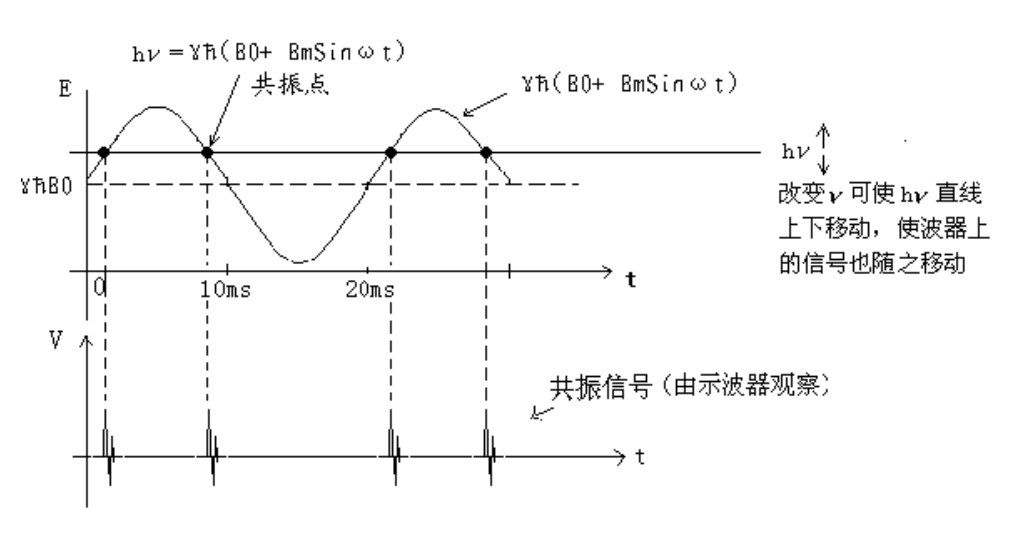
\includegraphics[width=0.7\textwidth]{./prin.png}
        \caption{实验方法示意图}
    \end{minipage}
\end{figure}

当满足$\omega_0 = \gamma (B_0+B_m \sin{100\pi t})$时会出现共振信号,且当共振信号等间距时,有$\omega_0 = \gamma B_m$

\section{实验内容}

\subsection{实验仪器}

\begin{figure}[H]
    \centering
    \begin{minipage}[b]{0.9\textwidth}
        \centering
        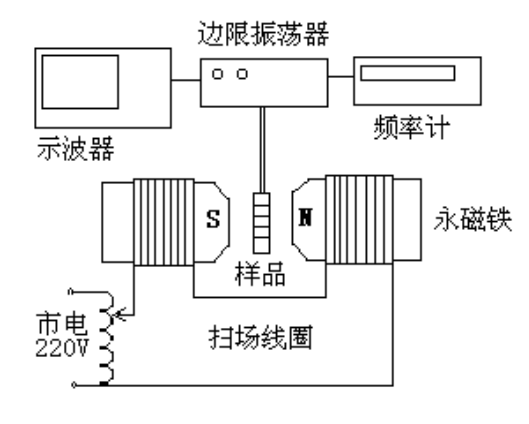
\includegraphics[width=0.5\textwidth]{./equip.png}
        \caption{实验仪器示意图}
    \end{minipage}
\end{figure}

\begin{enumerate}
    \item 样品水:提供实验用的粒子,$^1H,^{19}F$
    \item 永磁铁:提供稳恒外磁场$B_0$,中心磁感应强度约为0.58T。
    \item 边限振荡器:产生射频场,提供一个垂直于稳恒外磁场的高频电磁场频率(旋转
磁场 $B_1$)。同时也将探测到的共振电信号放大后输出到示波器,边限振荡器的频
率由频率计读出。
    \item 绕在永磁铁外的磁感应线圈:提供叠加在永磁铁上的调制场$B =B_m\sin{100\pi t}$
    \item 调压变压器:为磁感应线圈提供 50Hz 的可调电压。
    \item 频率计:读取射频场的频率。
    \item 示波器:观察共振信号。
\end{enumerate}

\subsection{具体实验内容}

\begin{enumerate}
    \item 观察并分析调制场$\tilde{B}$的大小和射频频率$\nu$对共振信号波形的影响
    \item 计算$\gamma_H,g_H,\gamma_F,g_F$
    \item 计算不同位置的磁场强度$B_0(x)$
    \item 测量5个不同调制电压下(0-100V)的$B_m$
\end{enumerate}

\section{原始实验数据}

{\bfseries 注:}系统显示是5号座位,实际在4号位置操作

\subsection{4号位置已知实验参数}

已知中心的磁场强度为$0.58T$。当样品处于磁场中心时,边限振荡器的右侧的刻度为$3.5cm$

\subsection{实验现象描述}

\subsubsection{调制场$\tilde{B}$的大小对共振信号波形的影响}

当增加接入的电压大时,调制场$\tilde{B}$的峰值$B_m$的变大。

发现,若在某时刻出现了共振信号,当射频频率不变的情况下,当$B_m$变大的时候共振信号的峰值也随之增加;而当$B_m$变小的时候,共振信号的峰值也随之减少,当$B_m$小于某个值时
共振信号消失。

\subsubsection{射频频率$\nu$对共振信号波形的影响}

发现,若在某时刻出现了共振信号,当调制场$\tilde{B}$不变的情况下,当$\nu$变大到某个值后,共振信号会重叠,再变大后则会消失;
当$\nu$变小到某个值后,共振信号会重叠,再变小后则会消失;当$\nu$取某个恰当的值时,会使共振信号变为等间距。

\subsection{数据记录表}

\begin{table}[H]
    \centering
    \begin{tabular}{|c|c|c|c|c|c|c|}
    \hline
        组数 & 1 & 2 & 3 & 4 & 5 & 6 \\ \hline
        $\nu /MHz$ & 24.620713 & 24.621753 & 24.621300 & 24.621067 & 24.621513 & 24.621501 \\ \hline
    \end{tabular}
    \caption{$^1H$核磁共振时频率计读数记录表}
\end{table}

\begin{table}[H]
    \centering
    \begin{tabular}{|c|c|c|c|c|c|c|}
    \hline
        组数 & 1 & 2 & 3 & 4 & 5 & 6 \\ \hline
        $\nu /MHz$ & 23.162852 & 23.163111 & 23.162131 & 23.162203 & 23.162103 & 23.162861 \\ \hline
    \end{tabular}
    \caption{$^{19}F$核磁共振时频率计读数记录表}
\end{table}

\begin{table}[H]
    \centering
    \begin{tabular}{|c|c|c|c|c|c|c|}
    \hline
        $\nu /MHz$ & 1 & 2 & 3 & 4 & 5 & 6 \\ \hline
        2cm & 24.618354 & 24.616727 & 24.617720 & 24.618302 & 24.618877 & 24.618675 \\ \hline
        3cm & 24.620753 & 24.620070 & 24.620269 & 24.620208 & 24.619898 & 24.619891 \\ \hline
        4cm & 24.622112 & 24.622933 & 24.621642 & 24.622159 & 24.622527 & 24.621783 \\ \hline
        5cm & 24.620847 & 24.622769 & 24.620229 & 24.621194 & 24.621755 & 24.622271 \\ \hline
    \end{tabular}
    \caption{不同位置(外磁场$B_0(x)$)下$^1H$核磁共振时频率计读数记录表}
\end{table}

说明,此处的$l$是边限振荡器右侧在磁体固定的刻度尺上的读数

\begin{table}[H]
    \centering
    \begin{tabular}{|c|c|c|c|c|c|}
    \hline
        电压V/v & 100 & 80 & 60 & 40 & 20 \\ \hline
        $\nu_1 /MHz$ & 24.582016 & 24.588243 & 24.596032 & 24.603952 & 24.611901 \\ \hline
        $\nu_2 /MHz$ & 24.659694 & 24.651687 & 24.644097 & 24.636851 & 24.629393 \\ \hline
    \end{tabular}
    \caption{不同调制电压下$^1H$核磁共振时频率计读数记录表}
\end{table}

\section{数据处理与数据分析}

\subsection{实验现象的解释}

产生共振信号需要满足的条件是:

\begin{equation}
    2\pi \nu = \gamma (B_0 + B_m \sin{100\pi t})
\end{equation}

\subsubsection{调制场$\tilde{B}$的大小对共振信号波形的影响}

改变$B_m$的大小会导致可能发生核磁共振的频谱范围发生了改变,在$\nu$不变的情况下,当$B_m$变大时,原来的核磁共振信号会变得更大,而当$B_m$变小时,信号会变弱,直到
$B_m$脱离了核磁共振的范围,此时核磁共振现象会消失,其信号自然也随之消失。

与观察的现象相符。

\subsubsection{射频频率$\nu$对共振信号波形的影响}

改变$\nu$的大小,就相当于改变了频率在频谱中的位置,在$B_m$不变的情况下,$\nu$的取值范围为$\nu \in \frac{\gamma}{2\pi}[B_0-B_m,B_0+B_m]$,当$\nu > \frac{\gamma}{2\pi}(B_0+B_m)$或$\nu < \frac{\gamma}{2\pi}(B_0-B_m)$时,核磁共振会消失,而当$\nu= \frac{\gamma}{2\pi}B_0$时,共振信号为等间距。

与实验现象相符。

\subsection{计算$\gamma_H,g_H,\gamma_F,g_F$}

计算得$\bar{\nu_H} = 24.621308 MHz,\bar{\nu_F} = 23.162544MHz$:

由$\gamma$和$g$的计算公式:

\begin{equation}
    \gamma = \frac{2\pi \bar{\nu}}{B_0}
\end{equation}

\begin{equation}
    g = \gamma \frac{\hbar}{\mu_{N}}
\end{equation}

其中$B_0 = 0.58T,\hbar = 1.0545718 \times 10^{-34} J\cdot s,\mu_N = 5.050783699 \times 10^{-27} J/T$

分别代入$^1H$和$^{19}F$中的数据得:

\begin{equation}
    \gamma_H = 2.667246\times 10^8 rad \cdot T^{-1}\cdot s^{-1}, \quad g_H = 5.569042
\end{equation}

\begin{equation}
    \gamma_F = 2.509216\times 10^8 rad \cdot T^{-1}\cdot s^{-1}, \quad g_F = 5.239086
\end{equation}

发现测得的旋磁比与朗德因子均与理论的值相近。

\subsection{计算不同位置的磁场强度$B_0(x)$}

得到不同位置处$\bar{\nu}$的值见下表:

\begin{table}[H]
    \centering
    \begin{tabular}{|c|c|c|c|c|}
    \hline
        位置$l/cm$ & 2 & 3 & 4 & 5 \\ \hline
        频率平均值$\bar{\nu}/MHz$ & 24.618109 & 24.620182 & 24.622193 & 24.621511 \\ \hline
    \end{tabular}
    \caption{不同位置处的频率平均值$\bar{\nu}$表}
\end{table}

由计算公式:

\begin{equation}
    B_0 = \frac{2\pi \bar{\nu}}{\gamma}
\end{equation}

得:

\begin{table}[H]
    \centering
    \begin{tabular}{|c|c|c|c|c|}
    \hline
        位置$l/cm$ & 2 & 3 & 4 & 5 \\ \hline
        磁感应强度$B_0/T$ & 0.579925 & 0.579973 & 0.580021 & 0.580005 \\ \hline
    \end{tabular}
    \caption{不同位置处的磁感应强度$B_0/T$表}
\end{table}

说明永磁铁中不同位置的磁场强度是不同的,是不均匀的。但大体上可认为在中心的磁场强度是均匀。

\subsection{测量5个不同调制电压下(0-100V)的$B_m$}

处理数据得:

\begin{table}[H]
    \centering
    \begin{tabular}{|c|c|c|c|c|c|}
    \hline
        电压V/v & 100 & 80 & 60 & 40 & 20 \\ \hline
        $(\nu_2-\nu_1) /MHz$ & 0.077678 & 0.063444 & 0.048065 & 0.032899 & 0.017492 \\ \hline
    \end{tabular}
    \caption{不同调制电压下$^1H$核磁共振时频率计读数差值记录表}
\end{table}

由计算公式:

\begin{equation}
    B_m = \frac{1}{2}(\frac{2\pi (\nu_2-\nu_1)}{\gamma}) = \frac{\pi (\nu_2-\nu_1)}{\gamma}
\end{equation}

得:

\begin{table}[H]
    \centering
    \begin{tabular}{|c|c|c|c|c|c|}
    \hline
        电压V/v & 100 & 80 & 60 & 40 & 20 \\ \hline
        $B_m/Gs$ & 9.149236 & 7.472697 & 5.661294 & 3.874980 & 2.060280 \\ \hline
    \end{tabular}
    \caption{不同调制电压下产生的磁场强度峰值$B_m$记录表}
\end{table}

发现不同调制电压产生的感应磁场磁感应强度峰值$B_m$是几乎呈线性的,是符合物理直观的。

\section{实验总结和误差分析}

\subsection{误差分析}

在实验中还存在一些问题:

\begin{enumerate}
    \item 观察共振信号是否等间距靠的是肉眼,会产生较大误差。
    \item 在测量不同位置的磁场强度时,在边缘的点$l=2cm,3cm$处。由于数字示波器不能检验到触发信号,图像无法锁定,故只能依靠模拟示波器进行粗略的估计,
    共振信号不一定等间距。
    \item 在利用频率计读数时,由于频率计示数在不断的跳动,所以会产生估读误差。
    \item 实验中可能还存在一些系统误差,但由于实验装置是集成的,这里无法分析。
\end{enumerate}

\subsection{实验总结}

\begin{enumerate}
    \item 调制场$\tilde{B}$的峰值$B_m$和射频频率$\nu$均会对共振信号波形产生影响,实验中需要寻找合适的值才能观察到现象。
    \item 实验中测得的$^1H,^{19}F$的旋磁比与朗德因子分别为
    $\gamma_H = 2.667246\times 10^8 rad \cdot T^{-1}\cdot s^{-1},g_H = 5.569042,\gamma_F = 2.509216\times 10^8 rad \cdot T^{-1}\cdot s^{-1},g_F = 5.239086$
    且发现测量值与理论值相近。
    \item 发现永磁铁中不同位置的磁感应强度是不同的,不太均匀,但大体上可认为中心磁感应强度是均匀的。
    \item 发现不同调制电压产生的感应磁场磁感应强度峰值$B_m$是几乎呈线性的,是符合物理直观的。
\end{enumerate}

\section{思考题}

\subsection{$B_0,B_1,\tilde{B}$的作用是什么?如何产生,它们有何区别?}

\begin{enumerate}
    \item $B_0$为稳恒外磁场,是为了使得原子核在外磁场的作用下产生Lamor进动。其由装置中的永磁铁产生。
    \item $B_1$为垂直于稳恒磁场方向的外加磁场,且绕稳恒磁场方向以角速度$\omega$旋转,是为了与外磁场中的原子核产生核磁共振。其由边限振荡器产生。
    \item $\tilde{B}$为沿稳恒磁场方向的外加交流磁场,且在本次实验中,其表达式为$\tilde{B} = B_m \sin{100\pi t}$,是为了增加能够观察到核磁共振现象的频谱范围,更加容易观察到核磁共振现象,且更加方便测量。其由
    围绕着永磁铁的且外加交流电的线圈产生。
\end{enumerate}

它们的区别由上分析显然得到,它们的目的和产生机制都是不同的。

\section{致谢}

感谢一教物理实验中心提供的核磁共振实验仪器,也感谢王少敏助教的指导!

\section{参考文献}

\begin{enumerate}
    \item 核磁共振实验实验讲义. 大学物理实验-现代物理实验.
\end{enumerate}

\end{document}